\section{Introduction}

As a free online service, VirusTotal~\cite{virustotal} analyzes files submitted by real-world users to identify many different kinds of malwares, 
like viruses, worms, trojans, and so on. 
VirusTotal applies different antivirus engines to each submitted file and generate an aggregated reports. 
All submitted files and generated reports are saved and can be accessed through public API. 


The repository on VirusTotal provides a good source to conduct data mining. 
Firstly, there are huge amount of data on VirusTotal.
Figure~\ref{fig:subnum} shows the number of distinct files submitted from XXX to XXX. 
We can see that there are XXX distinct suspicious files submitted each day. 
This amount of data makes VirusTotal a rough estimation of malwares in the real world. 
Secondly, all data on VirusTotal are labeled by state-of-the-art antivirus techniques. 
VirusTotal update each antivirus engine every 5 minutes. 
Besides whether a given a submitted file is detected by an antivirus engine, VirusTotal also keeps exact detection tag returned by each engine. 
There are also online active malware researchers, 
who can comment and vote each submitted file and serve as an important supplement of antivirus engines. 
We believe mining data on VirusTotal could enable many ``Big Security'' applications. 

In industry, antivirus vendors widely use VirusTotal to identify false negatives and false positives of their products. 
They only utilize VirusTotal reports for each single suspicious file, but fail to leverage the whole repository. 
In academia, researchers began to pay attention to correlations among different VirusTotal reports. 
For example, {\bf [ToDo: discuss Heqing's work]}
We believe there are much more research opportunities through mining VirusTotal. 

In this paper, we view data on VirusTotal as a stream, based on each submitted file’s ``first\_seen'' time, and design two stream mining applications: 
hot malware family mining and malware prediction. 
There are infinite possible malware families. 
Hot malware family mining can precisely identify malware families, 
which occupy more than a given percentage of total malwares, by using a constant number of counters.
We think malwares does not appear uniformly across different malware families or across time, 
and they appear in bursts. We built a cache-based algorithm to predict malwares in which families would appear in the near future. 

In summary, we made the following contributions in this paper:

\begin{itemize}

\item We study the characteristics of data on VirusTotal.
\item We design two data streaming applications.
\item We demonstrate the feasibiliy of mining VirusTotal data. 

\end{itemize}


\begin{figure}[t!]
\begin{center}
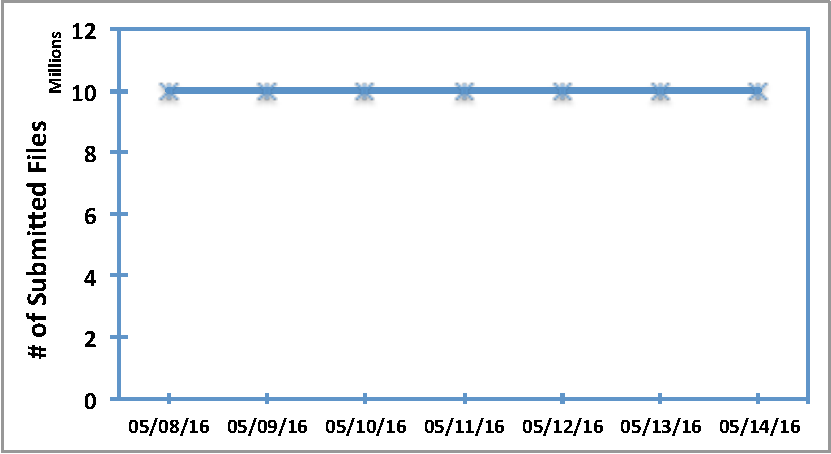
\includegraphics[width=3.2in]{figure/submission_number}
\caption{The number of files submitted to VirusTotal from 05/08/2016 to 05/14/2016. 
{\bf [TODO: All numbers in this figure are made up, and they must be changed later.]}}
\label{fig:subnum}
\end{center}
\end{figure}
